\section{Constructing an effective model}
\subsection{Pymablock workflow}

\co{The workflow of Pymablock consists of three steps.}
Building an effective model using Pymablock is a three step process:
%
\begin{itemize}
\item Define a Hamiltonian
\item Call \mintinline{python}|pymablock.block_diagonalize|
\item Request the desired order of the effective Hamiltonian
\end{itemize}
%
The following code snippet shows how to use Pymablock to compute the fourth
order correction to an effective Hamiltonian $\tilde{\mathcal{H}}$:
%
\begin{minted}{ipython}
from pymablock import block_diagonalize

# Define perturbation theory
H_tilde, *_ = block_diagonalize([H_0, H_1], subspace_eigenvectors=[vecs_A, vecs_B])

# Request 4th order correction to the effective Hamiltonian
H_AA_4 = H_tilde[0, 0, 4]
\end{minted}

\co{Depending on the input Hamiltonian, Pymablock uses specific routines to find
the effective model, so that symbolic expressions are compact and numerics are
efficient.}

The function \mintinline{python}|block_diagonalize| interprets the Hamiltonian $H_0 +
H_1$ and calls the block diagonalization routines depending on the
type and sparsity of the input.
This is the main function of Pymablock, and it is the only one that the user
ever needs to call.
It first output is a multivariate series whose terms are different blocks and
orders of the effective Hamiltonian.
Calling \mintinline{python}|block_diagonalize| is not computationally expensive, because the
terms of the series are only computed when requested.

\subsection{k.p model of bilayer graphene}

\co{We use bilayer graphene to illustrate how to use Pymablock with analytic models.}

To illustrate how to use Pymablock with analytic models, we consider two layers
of graphene stacked on top of each other.
Our goal is to find the low energy model near the $\mathbf{K}$ point
\cite{McCann_2013}.
First, we construct the Hamiltonian of bilayer graphene from its tight-binding
model.

\begin{figure}[!htbp]
\centering
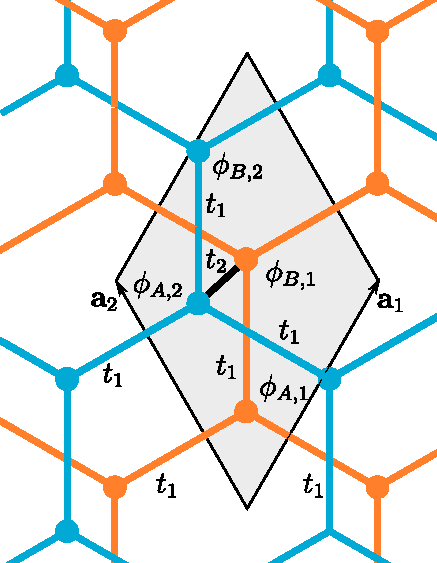
\includegraphics[width=0.3125\linewidth]{figures/bilayer_graphene.pdf}
\caption[]{Crystal structure and hoppings of bilayer graphene.}
\label{bilayer}
\end{figure}

The main features of the model are:
%
\begin{itemize}
\item The unit cell is spanned by vectors $\mathbf{a}_1 = (1/2, \sqrt{3}/2)$ and $\mathbf{a}_2=( -1/2, \sqrt{3}/2)$.
\item The unit cell contains 4 atoms with wave functions $\phi_{A,1}, \phi_{B,1}, \phi_{A,2}, \phi_{B,2}$.
\item The hoppings within each layer are $t_1$.
\item The hopping between atoms that are on top of each other is $t_2$.
\item The layers have an onsite potential $\pm m$.
\end{itemize}

\subsubsection{Defining a symbolic Hamiltonian}

We define the Bloch Hamiltonian using the Sympy package for symbolic Python
\cite{Meurer_2017}.
%
\begin{minted}{ipython}
import numpy as np
from sympy import symbols, Matrix, sqrt, Eq, exp, I, pi, Add, MatAdd
from sympy.physics.vector import ReferenceFrame

t_1, t_2, m = symbols("t_1 t_2 m", real=True)
alpha = symbols(r"\alpha")

H = Matrix([
    [m, t_1 * alpha, 0, 0],
    [t_1 * alpha.conjugate(), m, t_2, 0],
    [0, t_2, -m, t_1 * alpha],
    [0, 0, t_1 * alpha.conjugate(), -m]]
)
Eq(symbols("H"), H, evaluate=False)
\end{minted}

\begin{minted}{ipython}
Eq(H, Matrix([
[                    m, \alpha*t_1,                     0,          0],
[t_1*conjugate(\alpha),          m,                   t_2,          0],
[                    0,        t_2,                    -m, \alpha*t_1],
[                    0,          0, t_1*conjugate(\alpha),         -m]]))
\end{minted}
%
where $\alpha(\mathbf{k}) = 1 + e^{i \mathbf{k'} \cdot (\mathbf{a}_1 +
\mathbf{a}_2)}$ and $\mathbf{k'} = (4\pi/3 + k_x, k_y)$, because we choose
$\mathbf{K}=(4\pi/3, 0)$ as the reference point for the k.p effective model.

\subsubsection{Defining the perturbative series}

\co{We define the perturbative series}
To call \mintinline{python}|block_diagonalize|, we use the eigenvectors of the unperturbed
Hamiltonian at the $\mathbf{K}$ point.
To demonstrate the capabilities of Pymablock, we use $m$ as a perturbative
parameter too.
The unperturbed Hamiltonian is then $H(\alpha(\mathbf{K}) = m = 0)$, and its
eigenvectors are:
%
\begin{align}
v_{A,1} &= \begin{pmatrix} 1 \\ 0 \\ 0 \\ 0 \end{pmatrix} &
v_{A,2} &= \begin{pmatrix} 0 \\ 1 \\ 0 \\ 1 \end{pmatrix} &
v_{B,1} &= \frac{1}{\sqrt{2}} \begin{pmatrix} 0 \\ 0 \\ -1 \\ 1 \end{pmatrix} &
v_{B,2} &= \frac{1}{\sqrt{2}} \begin{pmatrix} 0 \\ 0 \\ 1 \\ 1 \end{pmatrix}
\end{align}
%
These determine the basis on which the perturbative corrections are computed
and $A$, the subspace of interest for the effective model.
Then, we substitute $\alpha(\mathbf{k})$ into the Hamiltonian, and define the
block diagonalization routine using that $k_x$, $k_y$, and $m$ are perturbative
parameters.
%
\begin{minted}{ipython}
from pymablock import block_diagonalize

H_tilde, U, U_adjoint = block_diagonalize(
    H.subs({alpha: alpha_k}),
    symbols=(k_x, k_y, m),
    subspace_eigenvectors=[vecs[:, :2], vecs[:, 2:]]
)
\end{minted}
%
The order of the variables in the perturbative series will be that of \mintinline{python}{symbols}.

\subsubsection{Requesting the effective Hamiltonian}

We need corrections up to third order in momentum to compute the standard
quadratic dispersion of bilayer graphene and trigonal warping.
Therefore, we define second and third order terms in momentum and group them
total power of momentum.
%
\begin{minted}{ipython}
k_square = np.array([[0, 1, 2], [2, 1, 0]])
k_cube = np.array([[0, 1, 2, 3], [3, 2, 1, 0]])
\end{minted}
%
Querying \mintinline{python}{H\_tilde} returns the results in a masked numpy array, so we
define \mintinline{python}{H\_tilde\_AA} to gather different entries into one symbolic expression.
Finally, the result is a symbolic expression of the effective Hamiltonian.
%
\begin{minted}{ipython}
mass_term = H_tilde_AA([0], [0], [1])
kinetic = H_tilde_AA(*k_square, 0)
mass_correction = H_tilde_AA(*k_square, 1)
cubic = H_tilde_AA(*k_cube, 0)
MatAdd(mass_term + kinetic, mass_correction + cubic, evaluate=False)
\end{minted}
%
\begin{minted}{ipython}
Matrix([
[                                                m, 3*t_1**2*( -k_x**2 - 2*I*k_x*k_y + k_y**2)/(4*t_2)],
[3*t_1**2*( -k_x**2 + 2*I*k_x*k_y + k_y**2)/(4*t_2),                                                -m]]) + Matrix([
[                                    3*m*t_1**2*( -k_x**2 - k_y**2)/(2*t_2**2), sqrt(3)*t_1**2*(k_x**3 - 5*I*k_x**2*k_y + 9*k_x*k_y**2 + 3*I*k_y**3)/(8*t_2)],
[sqrt(3)*t_1**2*(k_x**3 + 5*I*k_x**2*k_y + 9*k_x*k_y**2 - 3*I*k_y**3)/(8*t_2),                                      3*m*t_1**2*(k_x**2 + k_y**2)/(2*t_2**2)]])
\end{minted}
%
The first term contains the standard quadratic dispersion of bilayer graphene
with a gap.
The second term contains trigonal warping and the coupling between the gap and
momentum.

\subsection{Induced gap in a double quantum dot}

\co{Large systems pose an additional challenge due to the scaling of linear
algebra routines for large matrices.}
Large systems pose an additional challenge due to the cubic scaling of linear algebra
routines on matrices' size.
Pymablock handles large systems by using sparse matrices and avoiding the
construction of the full Hamiltonian.
We illustrate its efficiency with a model of two quantum dots coupled to a
superconductor between them.

\textit{(Include figure with scheme of the system)}

\subsubsection{Building the Hamiltonian with Kwant}

\co{We use Kwant to build the Hamiltonian of the system.}
We use the Kwant package \cite{Groth_2014} to build
the Hamiltonian of the system.
In the following code, we define a square lattice of $L \times W = 200 \times
40$ sites with 2 orbitals per unit cell.
The lattice is divided into three regions: a quantum dot on the left, a
superconducting region in the middle, and a quantum dot on the right.
%
\begin{minted}{ipython}
import tinyarray as ta
import matplotlib.backends
import scipy.linalg
from scipy.sparse.linalg import eigsh
import numpy as np
import kwant
import matplotlib.pyplot as plt
color_cycle = ["#5790fc", "#f89c20", "#e42536"]

from pymablock import block_diagonalize


sigma_z = ta.array([[1, 0], [0, -1]], float)
sigma_x = ta.array([[0, 1], [1, 0]], float)

syst = kwant.Builder()
lat = kwant.lattice.square(norbs=2)
L, W = 200, 40

def normal_onsite(site, mu_n, t):
    return ( -mu_n + 4 * t) * sigma_z

def sc_onsite(site, mu_sc, Delta, t):
    return ( -mu_sc + 4 * t) * sigma_z + Delta * sigma_x

syst[lat.shape((lambda pos: abs(pos[1]) < W and abs(pos[0]) < L), (0, 0))] = normal_onsite
syst[lat.shape((lambda pos: abs(pos[1]) < W and abs(pos[0]) < L / 3), (0, 0))] = sc_onsite
syst[lat.neighbors()] = lambda site1, site2, t: -t * sigma_z

def barrier(site1, site2):
    return (abs(site1.pos[0]) - L / 3) * (abs(site2.pos[0]) - L / 3) < 0

syst[(hop for hop in syst.hoppings() if barrier(*hop))] = (
    lambda site1, site2, t_barrier: -t_barrier * sigma_z
)
\end{minted}

The chemical potentials of the normal and superconducting regions are $\mu_n$
and $\mu_{sc}$, respectively, $\Delta$ is the superconducting gap, and $t$
is the hopping amplitude within each region.
The barrier strength between the quantum dots and the superconductor is
$t_{barrier}$, a parameter that we treat as a perturbation.
We will also consider the asymmetry of the dot potentials, $\delta \mu$, as a
perturbation.
%
\textbf{(Include figure with the system)}
%
The system is large: with this many sites even storing all the eigenvectors
would take 60 GB of memory.
Therefore, we use sparse matrices and compute only a few eigenvectors.
In this case, perturbation theory allows us to compute the effective
Hamiltonian of the low energy degrees of freedom.
%
To get the unperturbed Hamiltonian, we use the following values for $\mu_n$,
$\mu_{sc}$, $\Delta$, $t$, and $t_{\text{barrier}}$.
%
\begin{minted}{ipython}
params = dict(
    mu_n=0.05,
    mu_sc=0.3,
    Delta=0.05,
    t=1.,
    t_barrier=0.,
)

h_0 = syst.hamiltonian_submatrix(params=params, sparse=True).real
\end{minted}

The barrier strength and the asymmetry of the dot potentials are the two
perturbations that we vary.

\begin{minted}{ipython}
barrier = syst.hamiltonian_submatrix(
    params={**{p: 0 for p in params.keys()}, "t_barrier": 1}, sparse=True
).real
delta_mu = (
    kwant.operator.Density(syst, (lambda site: sigma_z * site.pos[0] / L)).tocoo().real
)
\end{minted}

\subsubsection{Define the perturbative series}

Since the Hamiltonian is large and we are only interested in the low energy
subspace, it is sufficient to compute the 4 lowest eigenvectors of the
unperturbed Hamiltonian.
These are the lowest energy Andreev states in two quantum dots.
%
\begin{minted}{ipython}
# %%time

vals, vecs = eigsh(h_0, k=4, sigma=0)
vecs, _ = scipy.linalg.qr(vecs, mode="economic")  # orthogonalize the vectors
\end{minted}
%
To orthogonalize the eigenvectors manually because
\mintinline{python}{scipy.sparse.linalg.eigsh} does not return orthogonal eigenvectors if the
matrix is complex and eigenvalues are degenerate.
%
We now define the block diagonalization routine and compute the few lowest
orders of the effective Hamiltonian.
Here we only provide the set of vectors of the interesting subspace.
This selects the \mintinline{python}{pymablock.implicit} method that uses efficient sparse
solvers for Sylvester's equation.
%
\begin{minted}{ipython}
# %%time

H_tilde, *_ = block_diagonalize([h_0, barrier, delta_mu], subspace_eigenvectors=[vecs])
\end{minted}
%
Block diagonalization is now the most time consuming step because it requires
pre-computing several decompositions of the full Hamiltonian.
It is, however, manageable and it only produces a constant overhead.

\subsubsection{Get the effective Hamiltonian}

For convenience, we collect the lowest three orders in each parameter in an
appropriately sized tensor.
%
\begin{minted}{ipython}
# %%time

# Combine all the perturbative terms into a single 4D array
fill_value = np.zeros((), dtype=object)
fill_value[()] = np.zeros_like(H_tilde[0, 0, 0, 0])
h_tilde = np.array(np.ma.filled(H_tilde[0, 0, :3, :3], fill_value).tolist())
\end{minted}
%
We see that we have obtained the effective model in only a few seconds.
We can now compute the low energy spectrum after rescaling the perturbative
corrections by the magnitude of each perturbation.
%
\begin{minted}{ipython}
def effective_energies(h_tilde, barrier, delta_mu):
    barrier_powers = barrier ** np.arange(3).reshape( -1, 1, 1, 1)
    delta_mu_powers = delta_mu ** np.arange(3).reshape(1, -1, 1, 1)
    return scipy.linalg.eigvalsh(
        np.sum(h_tilde * barrier_powers * delta_mu_powers, axis=(0, 1))
    )
\end{minted}
%
Finally, we plot the spectrum
%
\begin{minted}{ipython}
barrier_vals = np.array([0, 0.5, .75])
delta_mu_vals = np.linspace(0, 10e -4, num=101)
results = [
    np.array([effective_energies(h_tilde, bar, dmu) for dmu in delta_mu_vals])
    for bar in barrier_vals
]

plt.figure(figsize=(10, 6), dpi=200)
[
    plt.plot(delta_mu_vals, result, color=color, label=[f"$t_b={barrier}$"] + 3 * [None])
    for result, color, barrier in zip(results, color_cycle, barrier_vals)
]
plt.xlabel(r"$\delta_\mu$")
plt.ylabel(r"$E$")
plt.legend();
\end{minted}
%
% \includegraphics[width=0.7\linewidth]{files/95fc712be507bbaddfe033b24c38d25d.png}
%
As expected, the crossing at $E=0$ due to the dot asymmetry is lifted when the
dots are coupled to the superconductor. In addition, we observe how the
proximity gap of the dots increases with the coupling strength.
%
We also see that computing the spectrum perturbatively is faster than
repeatedly using sparse diagonalization for a set of parameters.
In this example the total runtime of Pymablock would only allow us to compute
the  eigenvectors at around 5 points in the parameter space.
